% !TEX root =  CCmoments.tex

\section{Blast Wave Model with a Full Hadron Gas and Comparison to STAR Results}\label{sec:blast}

The calculations of the previous section were based on a simple picture, where each sub-volume emitted particles whose probability of being observed was uniform, denoted by $\alpha$. In practice, this probability depends on where the sub-volume is located within the overall reaction volume. A sub-volume in the region with spatial rapidity, $|\eta_s|>1$, emits particles that are only rarely recorded by detectors that specialize in mid-rapidity measurements. Even for a sub-volume centered at mid-rapidity, thermal motion can spread some of its emission to rapidities outside the acceptance. This is especially true when the experiments narrow their acceptance. For example, STAR's acceptance nominally covers $\pm 1$ units of pseudo-rapidity, but the acceptance for identified particles is confined to $\pm 0.9$ units. For real rapidity, the effective acceptance is narrowed further, due to the fact that the true rapidity $y$ is less than the pseudo-rapidity $\eta$. This difference magnifies for massive, or slower particles. In fact, STAR analyses of identified particles often make cuts and only consider particles with true rapidities $-0.5<y<0.5$. Of course, even for particles within the rapidity acceptance, they must exceed some minimum transverse momentum and the efficiency for being detected is imperfect. For particles identified only by charge, the efficiencies are typically $\gtrsim 80\%$, and for identified particles the efficiency falls by another few tens of percent.

Collective flow plays a critical role. First, longitudinal flow is what allows the measurement of rapidity to correlate to a measurement in coordinate-space rapidity. In the Bjorken model of boost invariant flow, the mapping is simple in that a fluid element with spatial rapidity $\eta_s$ moves with a rapidity $\eta_s$, and particles emitted from a sub-volume with rapidity $\eta_s$ have rapidities $y\approx\eta_s$. This simple mapping is smeared by thermal motion. Collective radial flow and cooling combine to better align the spatial rapidity $\eta_s$ and the measured rapidity $y$. The thermal spread for pions is $\approx 0.6$ units of rapidity, while that for protons is $\approx 0.25$.

The size of the sub-volume clearly affects the result. If the sub-volume is small, there is an enhanced probability that a charge and its balancing charge will both be identified and cancel one another when assigning the net charge for an event. If the sub-volume extends over a large rapidity range, the effects of charge balance are minimized because there is a better chance that one charge will be observed while the other is outside the acceptance. The extent of the sub-volume in the transverse direction is less important. For sub-volumes at the edge of the fireball, which have more collective velocity, there is a modest increase of having balancing charges both pushed into the acceptance. The overall size also plays a role, as illustrated in the previous section, in that canonical suppression affects the results for smaller patch volumes. 

For the model in this section, canonical sub-volumes are overlaid onto a blast-wave model of collective flow. A filter is applied to the calculations, representing the experimental STAR acceptance and efficiency. This should be sufficiently realistic to make meaningful comparisons to STAR data. The four main parameters for the blast-wave model describe the radial flow $u_\perp$, the kinetic freeze-out temperature, $T_k$, and the baryon chemical potential and temperature at chemical freeze-out, $\mu_c$ and $T_c$. The chemical freeze-out temperature $\mu_c$ and chemical potential, $T_c$, are chosen to fit relative particle yields, while $T_k$ and $U_\perp$ are determined by simultaneously fitting the spectra of species with varying mass, typically $\pi,K,p$. A variety of parameterizations exist, such as having the velocity increase linearly from the origin, or the transverse rapidity, or having a sharp cutoff in radius vs. assuming a Gaussian profile. Depending on the choice, the value of $T_k$ and $u_\perp$ vary, but are typically in the neighborhood of $T_k\approx 100$ MeV and $u_\perp\approx 0.6$. For increasing multiplicities, the reaction volumes can expand and cool further, which leads to modestly increased values of $u_\perp$ and modestly decreased values of $T_k$ for either more central or for more energetic collisions. For this study the chemical freeze-out parameters were taken from \cite{Das:2012yq,Kumar:2012np}, which extracted $T_c$ and $\mu_c$ for a variety of beam energies. For this section, Bose statistics were ignored. Over 300 hadron species were included in the analysis. The collective flow velocities were chosen to reproduce the mean transverse momenta of both pions and protons.

The distributions of spatial rapidities, $\eta_s$, is chosen to be Gaussian, with a width $\sigma_0$ that depended on beam energy as
\begin{eqnarray}
\frac{dN}{d\eta_s}&\sim& e^{-\eta_s^2/2\sigma_0^2},\\
\nonumber
\sigma_0&=&0.4~y_{\rm beam},
\end{eqnarray}
where $\pm y_{\rm beam}$ are the rapidities of the incoming beams. This choice reproduces the rapidity widths measured at RHIC to roughly 10\% accuracy. The distribution of spatial rapidities for particles of a given patch was also spread according to a Gaussian with a width $\sigma_\eta$. The parameter $\sigma_\eta$ describes how far particles created from the same sub-volume may have separated by the time of emission. For increasingly larger values of $\sigma_\eta$, the chance that any two observed particles are correlated decreases.The rapidity of a patch was then distributed according to a Gaussian with width $\sqrt{\sigma_0^2-\sigma_\eta^2}$, so that the emission overall was characterized by the width $\sigma_0$. Whereas the other blast-wave parameters were chosen to describe spectra and yields, the parameter $\sigma_\eta$ is related to charge conservation. If charge is created early, and especially if the diffusion constant is large, the width might be of order unity, whereas if all the charge were to come after hadronization, the width might more likely be a few tenths. Blast-wave models of charge balance functions, which are also driven by charge conservation and diffusion, suggest widths should be of the order of a third, but variations of a factor of two were not ruled out \cite{Schlichting:2010qia}. One goal of this section is to investigate the sensitivity to $\sigma_\eta$.

For this blast-wave model, each sub-volume was also assigned a radial transverse velocity according to a Gaussian,
\begin{eqnarray}
\frac{dN}{d^2u_\perp}&\approx&e^{-(u_x^2+u_y^2)/2u_\perp^2}.
\end{eqnarray}
Each patch was also assigned a small spread in $\vec{u}_\perp$ , but given that, for this study, cuts are not being considered in transverse momenta or azimuthal angle, varying this parameter has little effect. 

The calculations of this section are filtered through a simplified model of the STAR detector's acceptance and efficiency. For unidentified particles, pseudo-rapidities are required to be less than 1.0 and transverse momenta are constrained to being above 150 MeV/$c$. An efficiency of 0.8 is applied. For identified particles, additional cuts are added. Rapidities are required to be less than 0.9 and transverse momenta are cut off above 1.5 GeV/$c$. The efficiency is lowered to 0.6. In order to compare results to measurement from STAR, the baryon densities and chemical freeze-out temperatures were mapped to beam energy according to the analysis of \cite{Kumar:2012np}, which extracted chemical freeze-out temperatures and chemical potentials by considering ratios of particle yields. The parameter, $u_\perp$, which controls the transverse radial flow was chosen along with the kinetic breakup temperature, $T_k$, to simultaneously roughly fit the mean transverse momenta of both the protons and pions reported \cite{Abelev:2009bw}. The kinetic freeze-out parameters were chosen according to the parameterization,
\begin{eqnarray}
T_k&=&120-20f~{\rm MeV},\\
u_\perp&=&0.5+(0.74-0.5)f,\\
f&=&\frac{1}{\ln(2)}
\ln\left[ 1+ \frac{\sqrt{s}-\sqrt{s}_0}{\sqrt{s}_f-\sqrt{s}_0}\right],
\end{eqnarray}
where $\sqrt{s}_0=7.7$ GeV and $\sqrt{s}_f=200$ GeV. Decays were simulated, and the products of weak decays (aside from pions or charged kaons) were included in the analysis. Undoubtedly, a more realistic model of the acceptance might change the ratios, but given that these are ratios, and that the overall efficiency and acceptances are not wildly off, a more rigorous model of the acceptance is unlikely to change the result by more than a few percent.

The summation over patches was performed by summing over 400 values of $u_\perp$ and $\eta_s$ consistent with the distributions described above. For each value, emission of $N_{\rm sample}=200$ thousand patches was simulated so that cumulants could be calculated for each value of $\eta_s$ and $u_\perp$. Because emission from different patches is uncorrelated, the cumulants for the total emission are simply the sum of the cumulants of each patch. Further, because the net cumulant behaves linearly in $N_{\rm sample}$, the ratios of net cumulants is independent of $N_{\rm sample}$.

\begin{figure}[htb]
\centerline{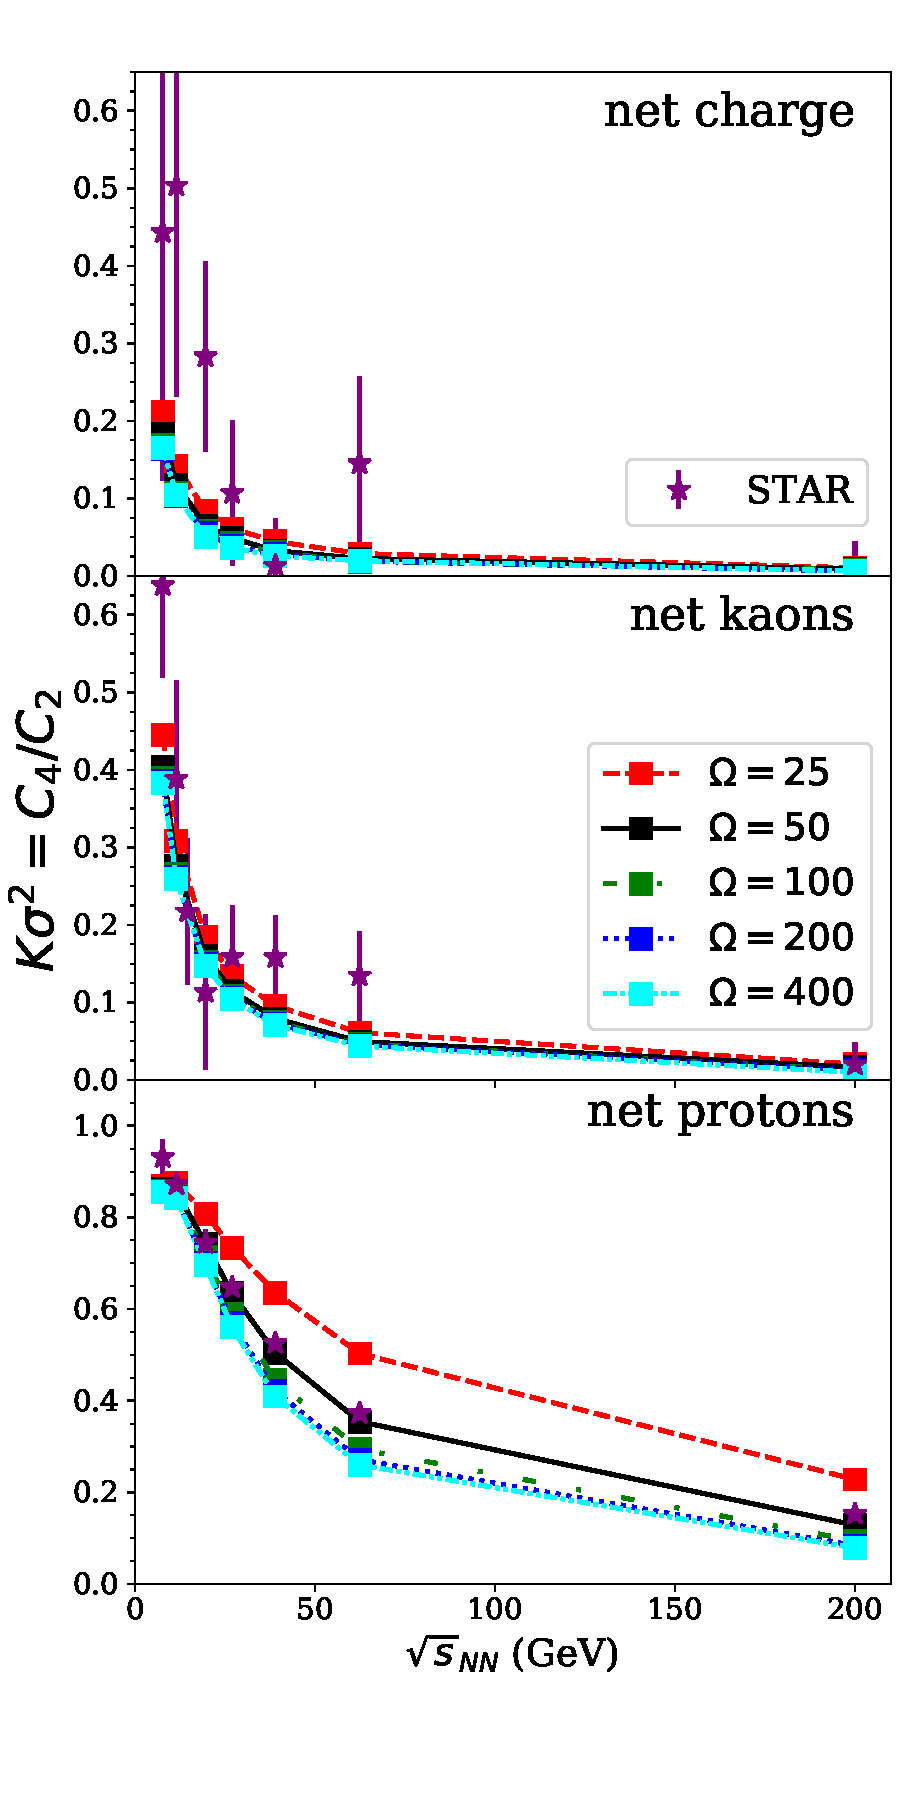
\includegraphics[width=0.45\textwidth]{figs/bw_skewness_omega}\hspace{0.06\textwidth}
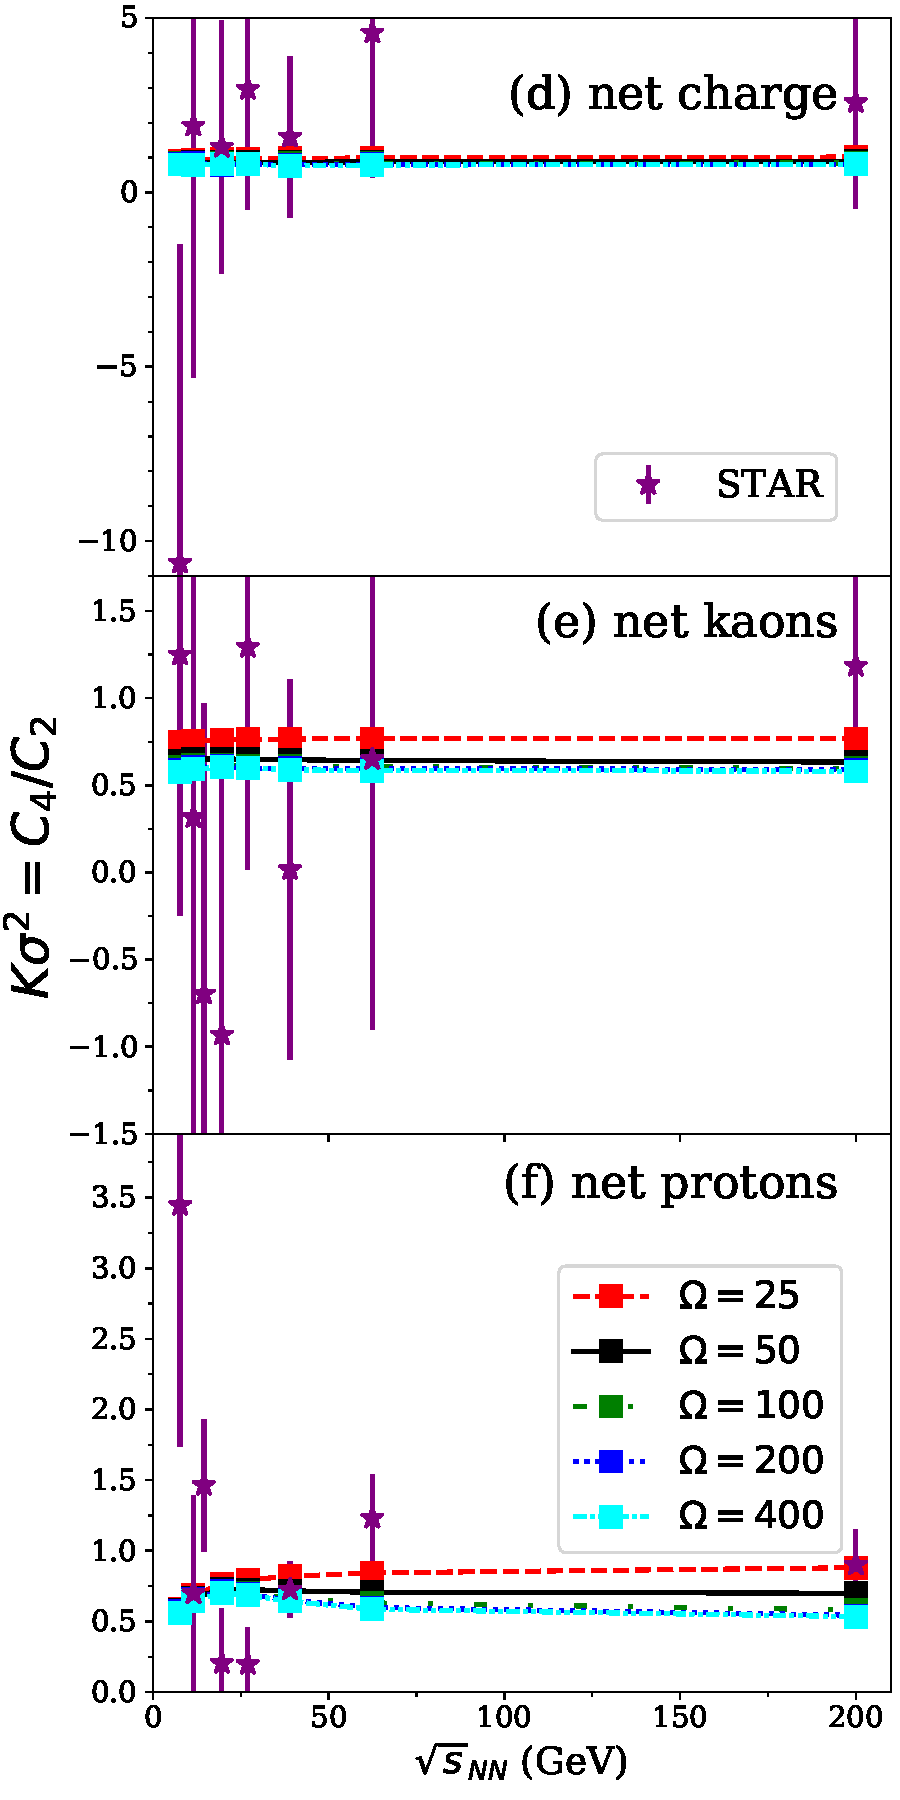
\includegraphics[width=0.45\textwidth]{figs/bw_kurtosis_omega}}
\caption{\label{fig:bw_vs_omega}(color online) The skewness (panels {\it a} and {\it b}) and kurtosis (panels {\it c} and {\it d}) are plotted for the blast wave models for different values of the sub-volume $\Omega$. For smaller sub-volumes the ratios $C_3/C_2$ and $C_3/C_1$ increase. For net charge, the ratios approach an asymptotic value once $\Omega$ begins to pass $\sim 50$ fm$^3$, whereas for net protons the ratios appear to approach the limit at somewhat higher values of $\Omega$. STAR measurements for net protons are not wholly dis-similar to the blast-wave calculations here, but those for net charge differ greatly. Additional physics from volume fluctuations might explain how $C_4/C_2$ might exceed unity, but it is difficult to explain how this might happen for net-charge distributions while leaving $C_4/C_2$ of the net-proton distribution unchanged.}
\end{figure}
Figure \ref{fig:bw_vs_omega} illustrates how results are sensitive to the size of the sub-volume. For these calculations $\sigma_\eta$ was fixed at 0.3. For a volume of 100 fm$^3$ the average number of hadrons is several dozen. For small sub-volumes, where in a grand canonical ensemble the typical number of charges would be zero or one, the thermodynamic cost of having a second charge to balance the first charge reduces the probability of having any charges. As mentioned earlier this is known as canonical suppression, and it lowers both the multiplicities and the moments. For larger sub-volumes, this thermodynamic cost vanishes as the system might have had fewer balancing charges of the same sign, rather than an extra balancing charge of the opposite sign. The characteristic volume for the disappearance of canonical suppression is the volume where the mean number of pairs exceeds unity. For charged particle this sets in at around 10 fm$^3$, but for baryons the characteristic volume is closer to 100 fm$^3$ because of their being heavier and fewer. Thus, the baryon moments for volumes of 50 fm$^3$ and 200 fm$^3$ differ more noticeably. The time for a fluid element to expand and cool to the point where it reaches chemical freeze-out tends to be on the order of 5 fm/$c$. These times are shorter for matter on the periphery, at a lower beam energy or at less centrality. The times are longer for a fluid element at the center, at higher beam energy, or in a more central collision. The maximum transverse distance a charge can travel before chemical freeze-out is 10 fm if they move in opposite directions, and if charge moves diffusively or if the charge is created later in the reaction, the separation should be significantly less. As discussed below, charge can separate further along the beam axis, and because that is not well understood, the size of the sub-volume carries a large uncertainty. Anywhere from 50 fm$^3$ to a few hundred fm$^3$ might be reasonable. 

Charge can spread further in the longitudinal direction due to the strong initial longitudinal collective flow at early times. This enhancement to the separation depends sensitively on when charge pairs are created. Matter thermalizes at a point with large collective velocity gradients along the beam axis. If the motion is diffusive, the separation along the beam axis depends logarithmically on the ratio of the final time to the initial creation time \cite{Bass:2000az}.  Thus, if a pair is created at 0.2 fm/$c$, the separation for times, $0.2<\tau<1.0$ fm/$c$ is as important as the additional separation they gain during the times $1.0<\tau<5.0$ fm/$c$. For this reason the size of charge spread, $\sigma_\eta$, in spatial rapidity might be anywhere between a few tenths of a unit of rapidity to a full unit. Figure \ref{fig:bw_vssigmaeta} shows the sensitivity of the moments to this parameter. For large $\sigma_\eta$ the observation of a charge is less likely to influence the observation of a second charge, which is similar to having a lower efficiency. For low efficiencies one expects the behavior to behave more like a Poissonian, and that $C_4/C_2$ and $C_3/C_1$ would be be closer to unity. Indeed, this is the case, but the dependence on $\sigma_\eta$, as shown in Fig. \ref{fig:bw_vs_sigmaeta}, is negligible for net charge and modest for net protons.
\begin{figure}
\centerline{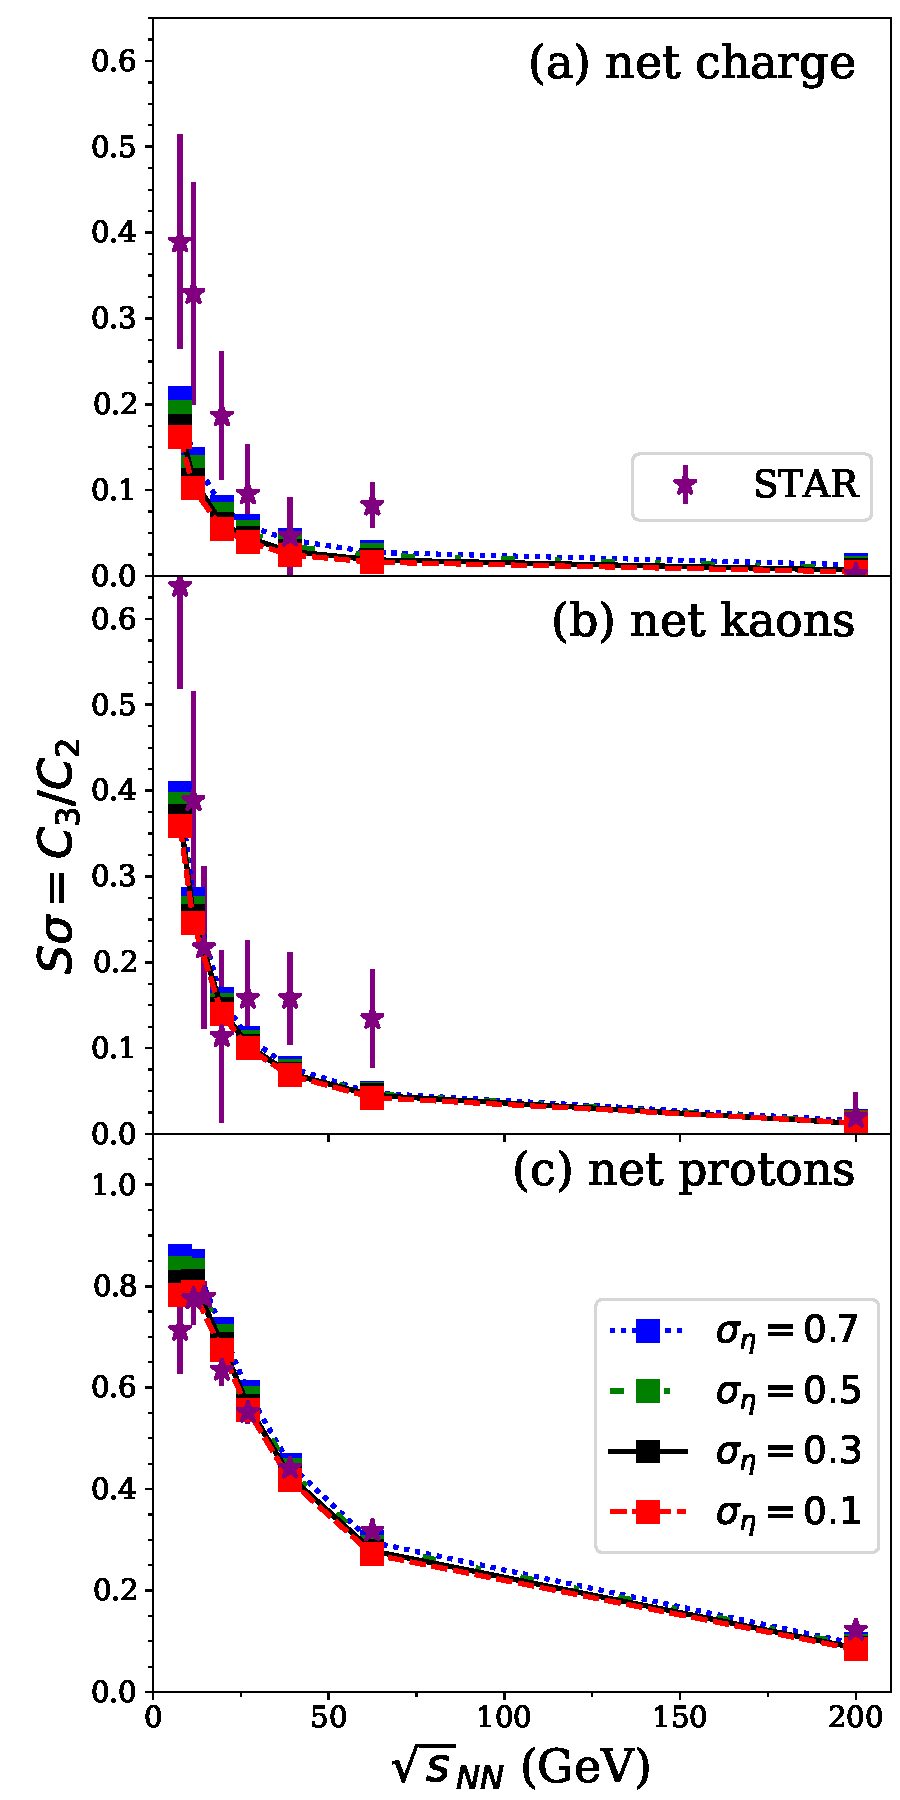
\includegraphics[width=0.45\textwidth]{figs/bw_skewness_sigmaeta}\hspace{0.06\textwidth}
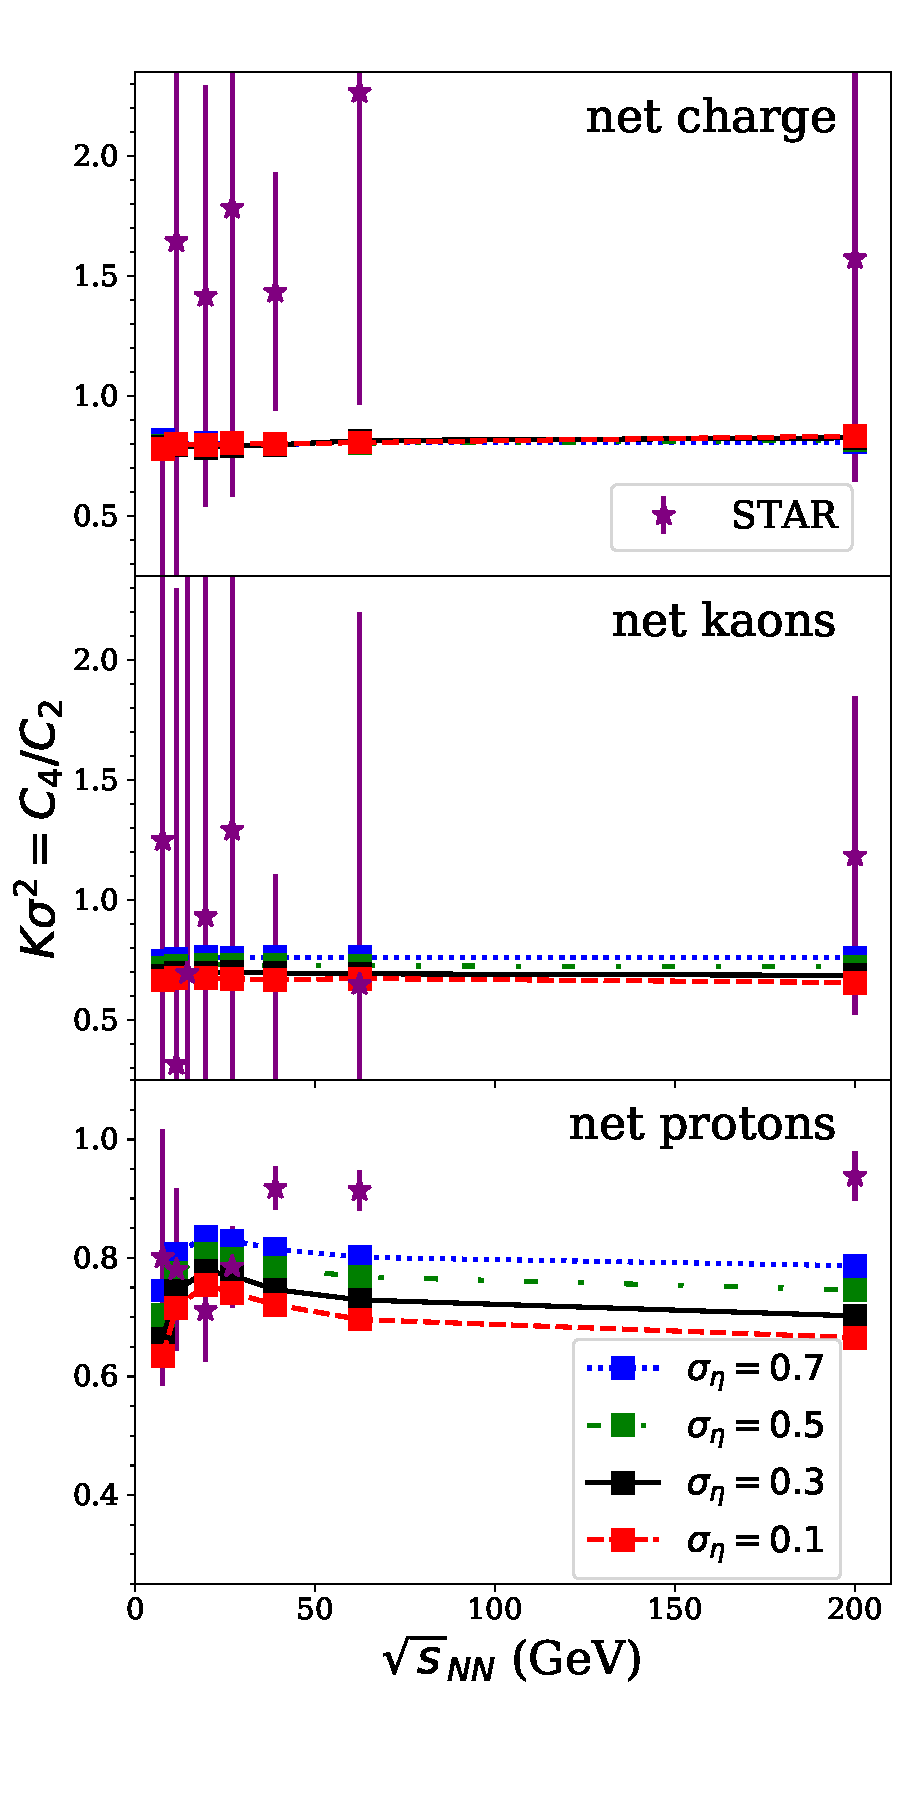
\includegraphics[width=0.45\textwidth]{figs/bw_kurtosis_sigmaeta}}
\caption{\label{fig:bw_vs_sigmaeta} (color online)  }
\end{figure}

The beam energy dependence mainly derives from the fact that the baryon density is higher for lower beam energies. The skewness, $C_3/C_2$, mus approach zero when the baryon density vanishes, and in the limit that there are no anti-baryons, the assumption that the baryons are deposited into the sub-volumes according to a Poissonian distribution drives $C_3/C_2$ for net protons to unity at high baryon density. Given the large number of charges, mainly in pions and kaons, relative to the number of protons and antiprotons, the imbalance of net charge due to the presence of stopped protons represents a smaller asymmetry to the net charge than it provides to the net protons. Thus, $C_3/C_2$ is closer to zero for net kaons or for net charge than it is for net protons. The sensitivity to $\Omega$, shown in Fig. \ref{fig:bw_vs_omega}, or to $\sigma_\eta$, illustrated in Fig. \ref{fig:bw_vs_sigmaeta}, is also more pronounced for net protons than for net kaons or for net charge.

The kurtosis, or $C_4/C_2$ ratio, varies only modestly with beam energy. For net charge, the ratio does not vary far from 0.8 in model calculations. In contrast, $C_4/C_2$ from model calculations for net protons varies from 0.6 to 0.9 depending on the values of $\Omega$ and $\sigma_\eta$. Experimental values are better reproduced with smaller sub-volumes, e.g. $\Omega\approx 50$ fm$^3$. The models also exhibit a dependence on beam energy for $C_4/C_2$. The ratio rises approximately 20 percent as the beam energy increases to 20 $A$GeV, then plateaus and falls 10\% until it becomes flat.

Figures \ref{fig:bw_vs_omega} and \ref{fig:bw_vs_sigmaeta} also display results from the STAR Collaboration for data recorded for central collisions, 0-5\% centrality. For the net proton fluctuations, the model results are similar to the STAR measurements for central collisions. The size and trend of $C_3/C_2$ as a function of beam energy is well reproduced, especially if smaller values of $\Omega$ are assumed. The trend of falling $C_3/C_2$ with increasing beam energy is mainly driven by the changing fraction of baryons that come from the creation of baryon-antibaryon pairs, vs. those that were deposited during the initial collision. As stated above this leads to the expectation that $C_3/C_2$ would be unity in the limit that anti-particles are ignored and all the deposited charge is deposited randomly, i.e. according to a Poissonian. Indeed baryons far exceed anti-baryons and low density and the ratio $C_3/C_2$ for net protons is near unity for both the model and data at low beam energy. At higher beam energies the number of baryons and antibaryons become more equal and $C_3/C_2$ goes to zero. The model rather well reproduces the experiment, especially if smaller values of $\Omega$, $\approx 50$ fm$^3$ are assumed. The ratio $C_4/C_2$ for net protons measured by STAR is also in line with the models, and again it better matches for smaller values of $\Omega$ are assumed. Unfortunately, due to the size of the error bars, the data cannot validate the rise and fall with beam energy seen in the models. 

The experimental results for net kaons are plagued by large statistical uncertainties. It would appear both $C_3/C_2$ and $C_4/C_2$ lie above the range of model predictions, but the error bars forbid one from making a strong conclusion. However, for net charge, one can clearly state that the observed cumulant ratios are incompatible with the model. Even with the large uncertainties, it is clear that the experimental ratios are well above unity. In fact, one expects that the model should always give ratios below unity for $C_4/C_2$, regardless of the choice of parameters. Much of the discussion in the upcoming summary, Sec. \ref{sec:summary}, centers on this failure.



